\section{Evaluation} \label{evaluation} 
To evaluate our continuous training approach, we perform several experiments.
We first describe the setup of our experiments including the computing cluster, the deployed pipeline, and how we simulate a real production environment by streaming a real-world large dataset through our deployment platform.
We discuss the effect of different parameters (learning rate adaptation, sampling strategy, and scheduling policy) on the quality and training time of the model.
Then, we discuss the effects of proactive training on the quality and freshness of the model and compare them to a model that is trained periodically.
Finally, we evaluate the training time of the continuous training approach and the effects of online statistics computation and data materialization optimizations on the training time.

\subsection{Setup}\label{subsec:setup}
We evaluate our deployment method in a distributed environment consists of 21 nodes (1 master, 20 slaves).
Each node is running on an Intel Xeon 2.40 GHz 16 core processor and has 28 GB of dedicated memory for running our prototype.
We use Apache Spark 2.2.0 running on Hadoop 2.7.
Each executor node has 16 task slots (a total of 320 slots).

To demonstrate the deployment platform, we designed the following machine learning pipeline and simulation:

\textbf{Criteo Pipeline.} 
The Criteo pipeline consists of 5 operations: input parser, missing value imputer, standard scaler, one hot encoder, and logistic regression model trainer. 
The Terabyte Criteo click log dataset is used for benchmarking algorithms for clickthrough rate (CTR) prediction \cite{criteo-log}.
It contains 24 days of user click logs. 
The dataset contains 13 numerical and 26 categorical features. 
In all of our experiments, we are using the data from the first 3 days (Day 0 to Day 2) of the Criteo dataset.
Day 0 is used for the initial offline training of the pipeline.
The data from Day 1 and Day 2 are used as streaming data sources.
To evaluate the quality of the pipeline, we use a sample of Day 6 to compute the logistic loss.

\textbf{Criteo Data Simulation.}
We simulate a production environment by streaming 2 days of the Criteo dataset.
The data from each day is divided into 1440 smaller batches and stored on disk.
Each batch represents one minute of data.
We use spark streaming to read the data files one by one and stream them through the deployment platform. 
All the experiments are using Day 1 and Day 2 as streaming sources unless specified otherwise.

\subsection{Learning Rate Adaptation Method}
In Section \ref{sgd}, we discussed the importance of learning rate tuning for training a model using the Stochastic Gradient Descent (SGD) optimization method.
Proactive training is an extension of SGD, and therefore the process of tuning the learning rate adaptation method is not different from tuning it for an offline SGD training.

To find the best learning rate adaptation algorithm, we first train a model using SGD optimization algorithm for 500 iterations using Adadelta, RMSprop, and Adam, three of the state-of-the-art learning rate adaptation techniques.
After the training, the models (and the pipelines) trained with different learning rate adaptation techniques are deployed.
We use the first day of the Criteo data to investigate the effect of the learning rate adaptation techniques on the Criteo pipeline.
Figure \ref{fig:criteo-learning-rate} shows the logistic loss error rate of different learning adaptation techniques. 
During the SGD training phase, we capture the logistic loss on the evaluation dataset after 20, 40, 80, 160, 320, and 500 iterations of training.


\begin{figure}[h!]
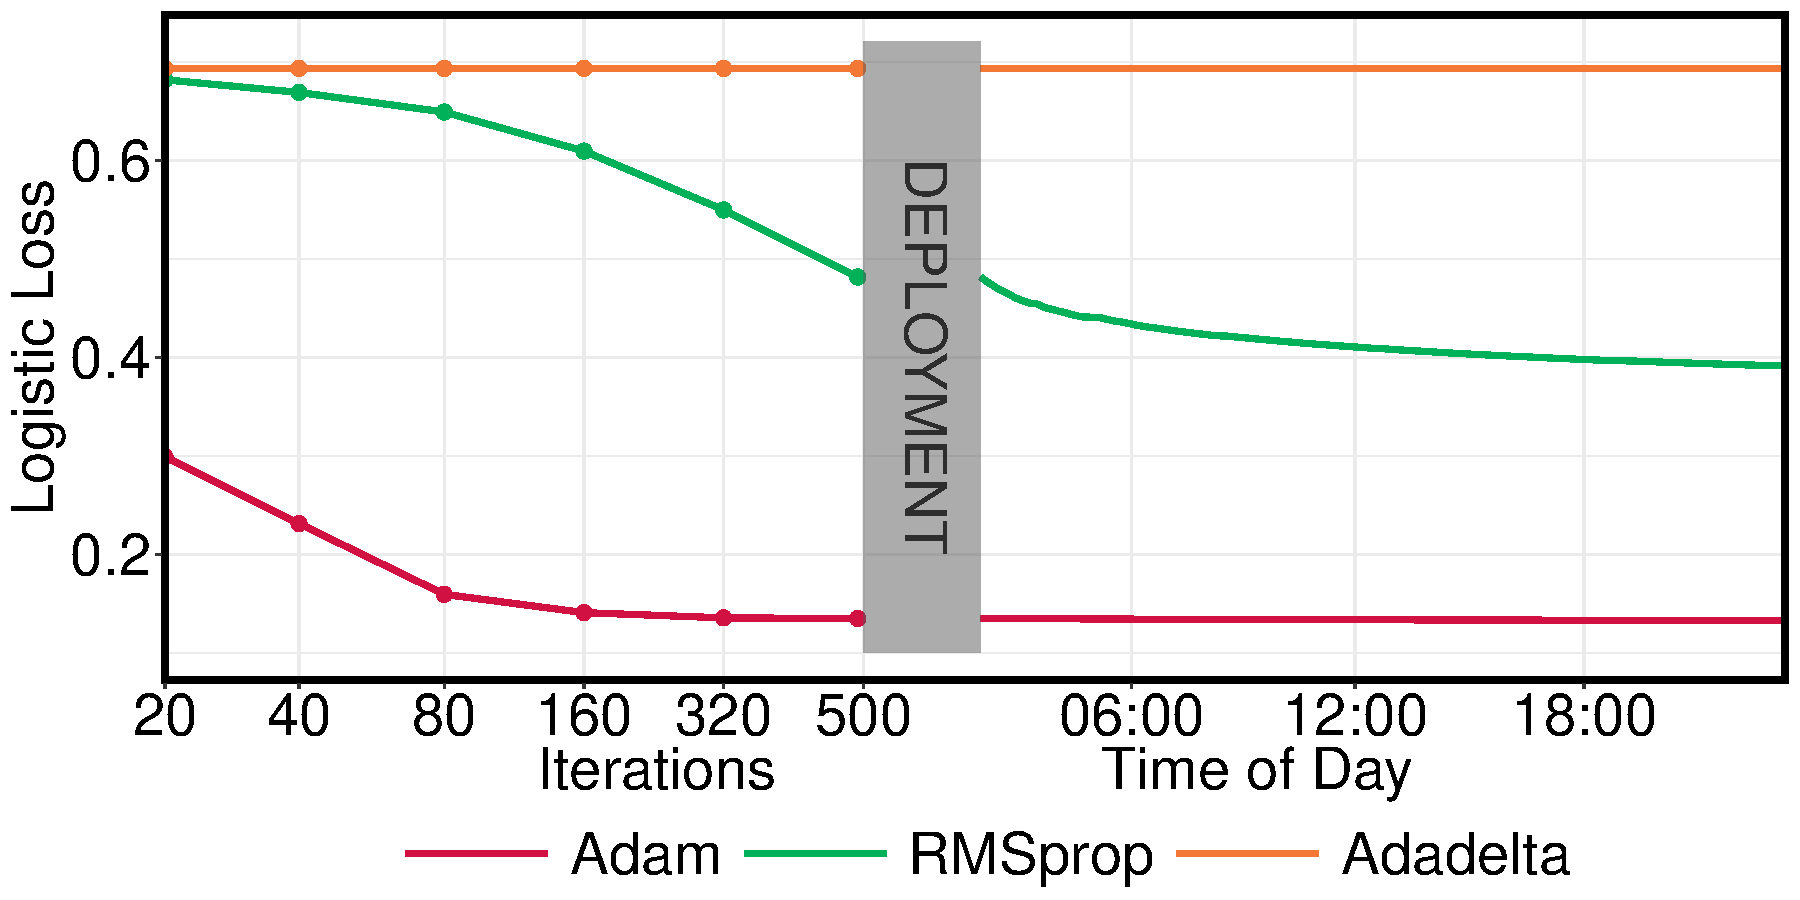
\includegraphics[width=\columnwidth]{../images/experiment-results/criteo-learning-rate-experiment.pdf}
\caption{Learning rate adaptation techniques for Criteo pipeline}
\label{fig:criteo-learning-rate}
\end{figure}

Adadelta performs very poorly during the offline training phase.
The Criteo dataset is a complex and high-dimensional data, where features are a mix of numerical and categorical variables.
Since categorical features are not standardized, Adadelta is not able to effectively tune the learning rate for a mix of standardized and non-standardized features.
Similar to the offline SGD training, Adadelta performs poorly for proactive training after the model is deployed.
In fact, the error rate of the model, starting from the 20th iteration to end of Day 1, stays almost constant throughout the experiment.

Unlike Adadelta, RMSprop reduces the error rate on the evaluation dataset through the offline SGD training.
Before the deployment, the error rate of the model is dropped to $0.48$.
Similarly, after the deployment, proactive training of the model using RMSprop reduces the error rate by $18\%$.

Adam has the best performance among the evaluated learning rate adaptation techniques.
Using Adam, the model fully converges after 500 iterations of SGD during the offline training phase.
After the deployment, the error rate is further reduced by $1.4\%$.
While the reduction in error rate for Adam is smaller than RMSprop, Adam still outperforms RMSprop after a day of proactive training of the model.

This experiment shows that process of selecting the learning rate adaption technique for proactive training is similar to the process of selecting it for the offline SGD training.
A learning rate adaptation technique that performs best during the offline training of the model also has the best performance for proactive training, when the model is deployed.

Even though Adam performs best for the Criteo pipeline, this does not indicate that Adam is the best learning rate adaptation technique for proactive training for every other pipeline and model.
For every pipeline and dataset, the users have to evaluate the performance of the different learning rate adaptation techniques during the offline training of the model.
The method that performs best during the offline training also has the best performance for the proactive training.

\subsection{Sampling Methods}
In this section, we analyze the effect of different sampling techniques on both the quality and the training time of the pipeline.
We use a sampling rate of $0.1\%$ for all of the experiments where a sampling is performed.
This sampling rate is chosen to be equal to the sampling rate used during the initial offline SGD training of the model.

Figure \ref{fig:sampling-mode-quality} shows how different sampling modes, namely random sampling, time-based sampling, and no sampling, affect the quality of the model in the Criteo pipeline.
In both random sampling and time-based sampling modes, first the data is sampled and then the new training data that has arrived at the system recently is appended to this sample and used in the proactive training.
In no sampling mode, only the recently arrived data is used in the proactive training.
In random sampling approach, the entire historical data is used for creating the sample.
In this scenario, the logistic error rate decreases in a very slow manner over time.
Since the deployed model is already fully trained on the historical data, using the historical data in the continuous training of the model does not have a big impact on the model quality.

\begin{figure}[h!]
\centering
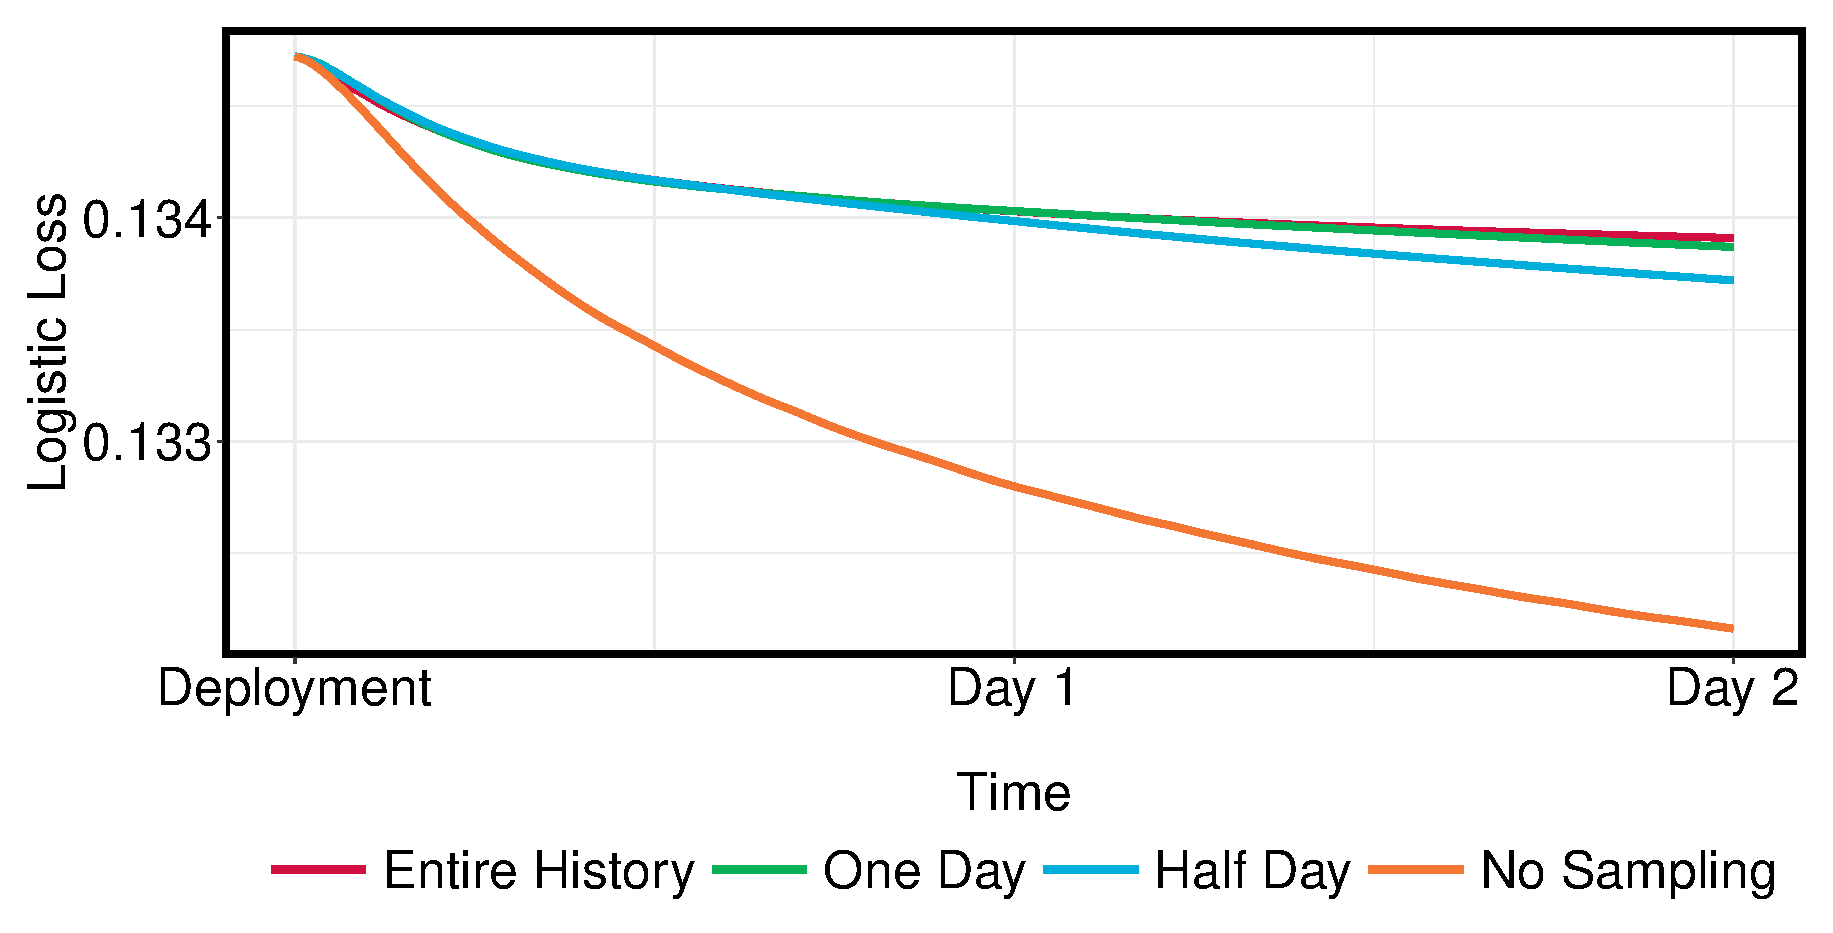
\includegraphics[width=\columnwidth]{../images/experiment-results/criteo-sampling-mode-experiments.eps}
\caption{Effect of different sampling modes on quality}
\label{fig:sampling-mode-quality}
\vspace{2mm}
\end{figure}

The time-based sampling has a larger impact on the quality of the model.
We evaluated the quality of the model for one day and half day time intervals.
Using an interval of one day, the time-based sampling decreases the error rate by 0.03\%  more than when using the simple random sampling (entire historical data).
Moreover, decreasing the interval length further, results in a model with lower logistic error rate.
In our experiment, using a time interval of half day for the time-based sampling results in an error rate that is 0.14\% smaller than when using the simple random sampling. 
Reducing the time interval in the time-based sampling limits the data in the sample to the more recently generated data, which allows the model to fit to more unseen and more time-relevant data.
In the Criteo pipeline, disabling sampling completely has the biggest impact on the error rate.
By not sampling the data, the error rate of the mode is decreased by $1.9\%$ over the two day deployment period.

This experiment shows that the sampling time interval has a big impact on the quality of the deployed model.
For Criteo pipeline, the dataset has a stable distribution, which stays the same throughout the course of the experiment.
As a result, limiting the training to the more recent data exposes the model to newer and unseen data which results in bigger changes (toward convergence) in the weights of the model (e.g., no sampling).
When the distribution of the incoming training data is stable, using more historical data to continuously train the model has little effect as the combination of historical and new data dampens the effects of the new data on the model (e.g., sampling from the entire history).
As a result, the improvement in the model convergence is very small.

\begin{figure}[h]
\begin{subfigure}{\columnwidth/2}
\centering
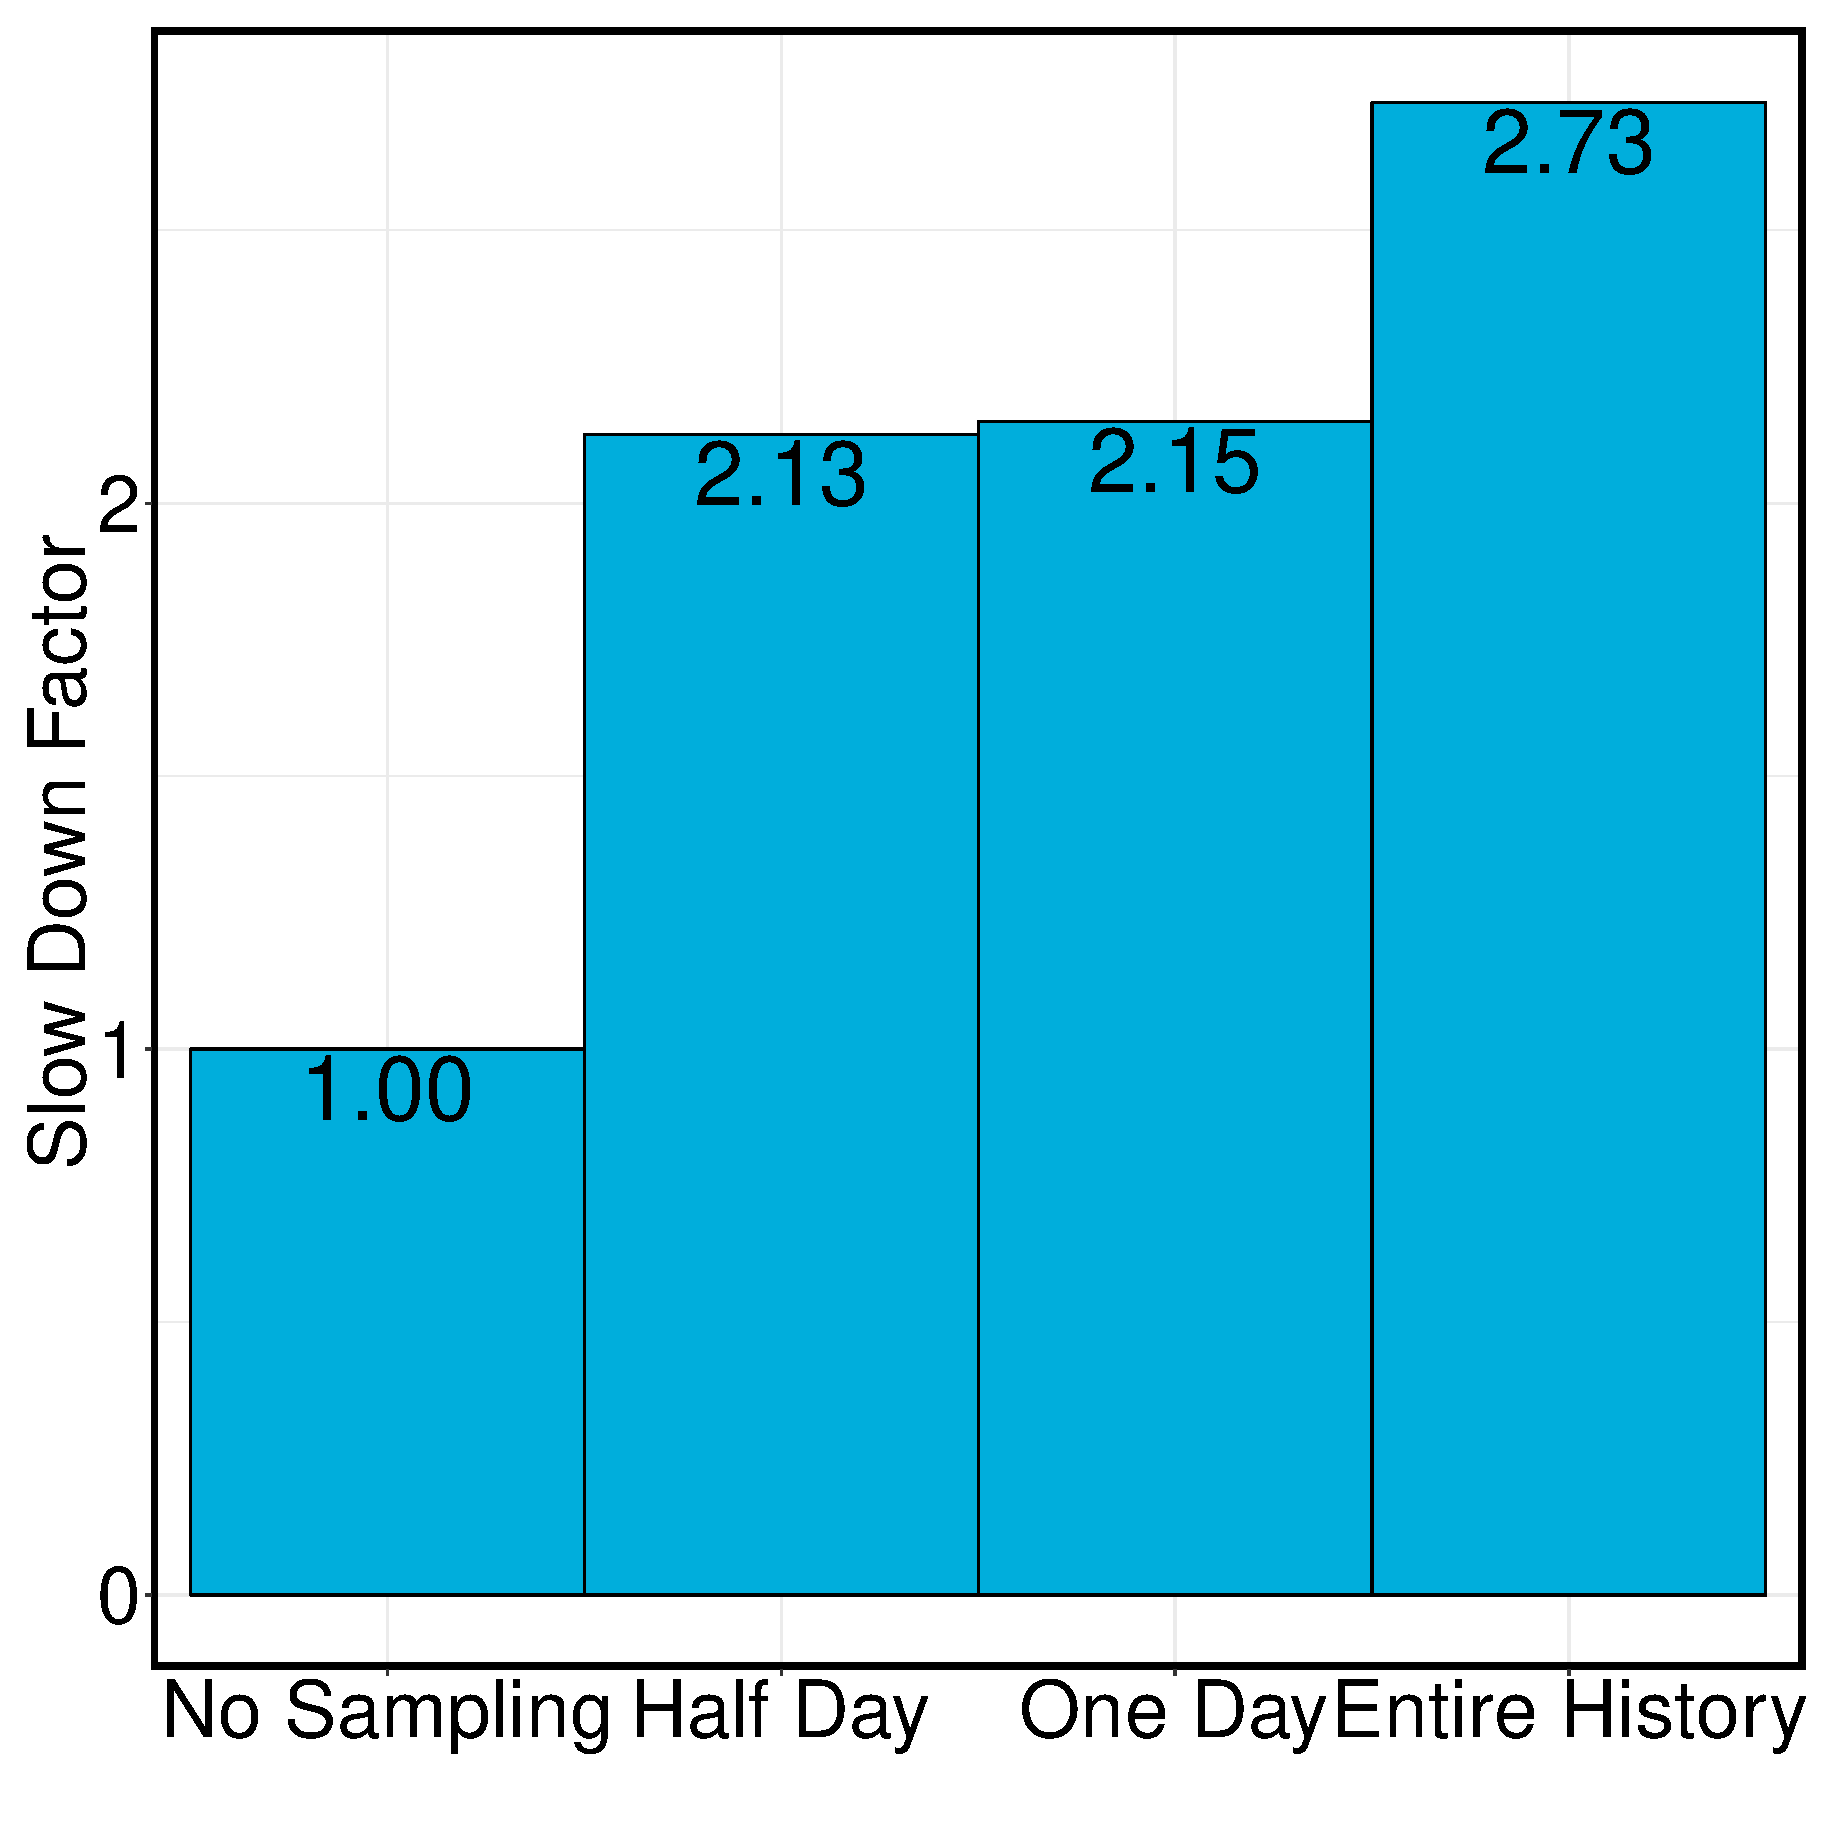
\includegraphics[width=\columnwidth]{../images/experiment-results/criteo-sampling-total-experiment.eps}
\caption{Total time}
\label{fig:sampling-mode-total-time}
\end{subfigure}%
\begin{subfigure}{\columnwidth/2}
\centering
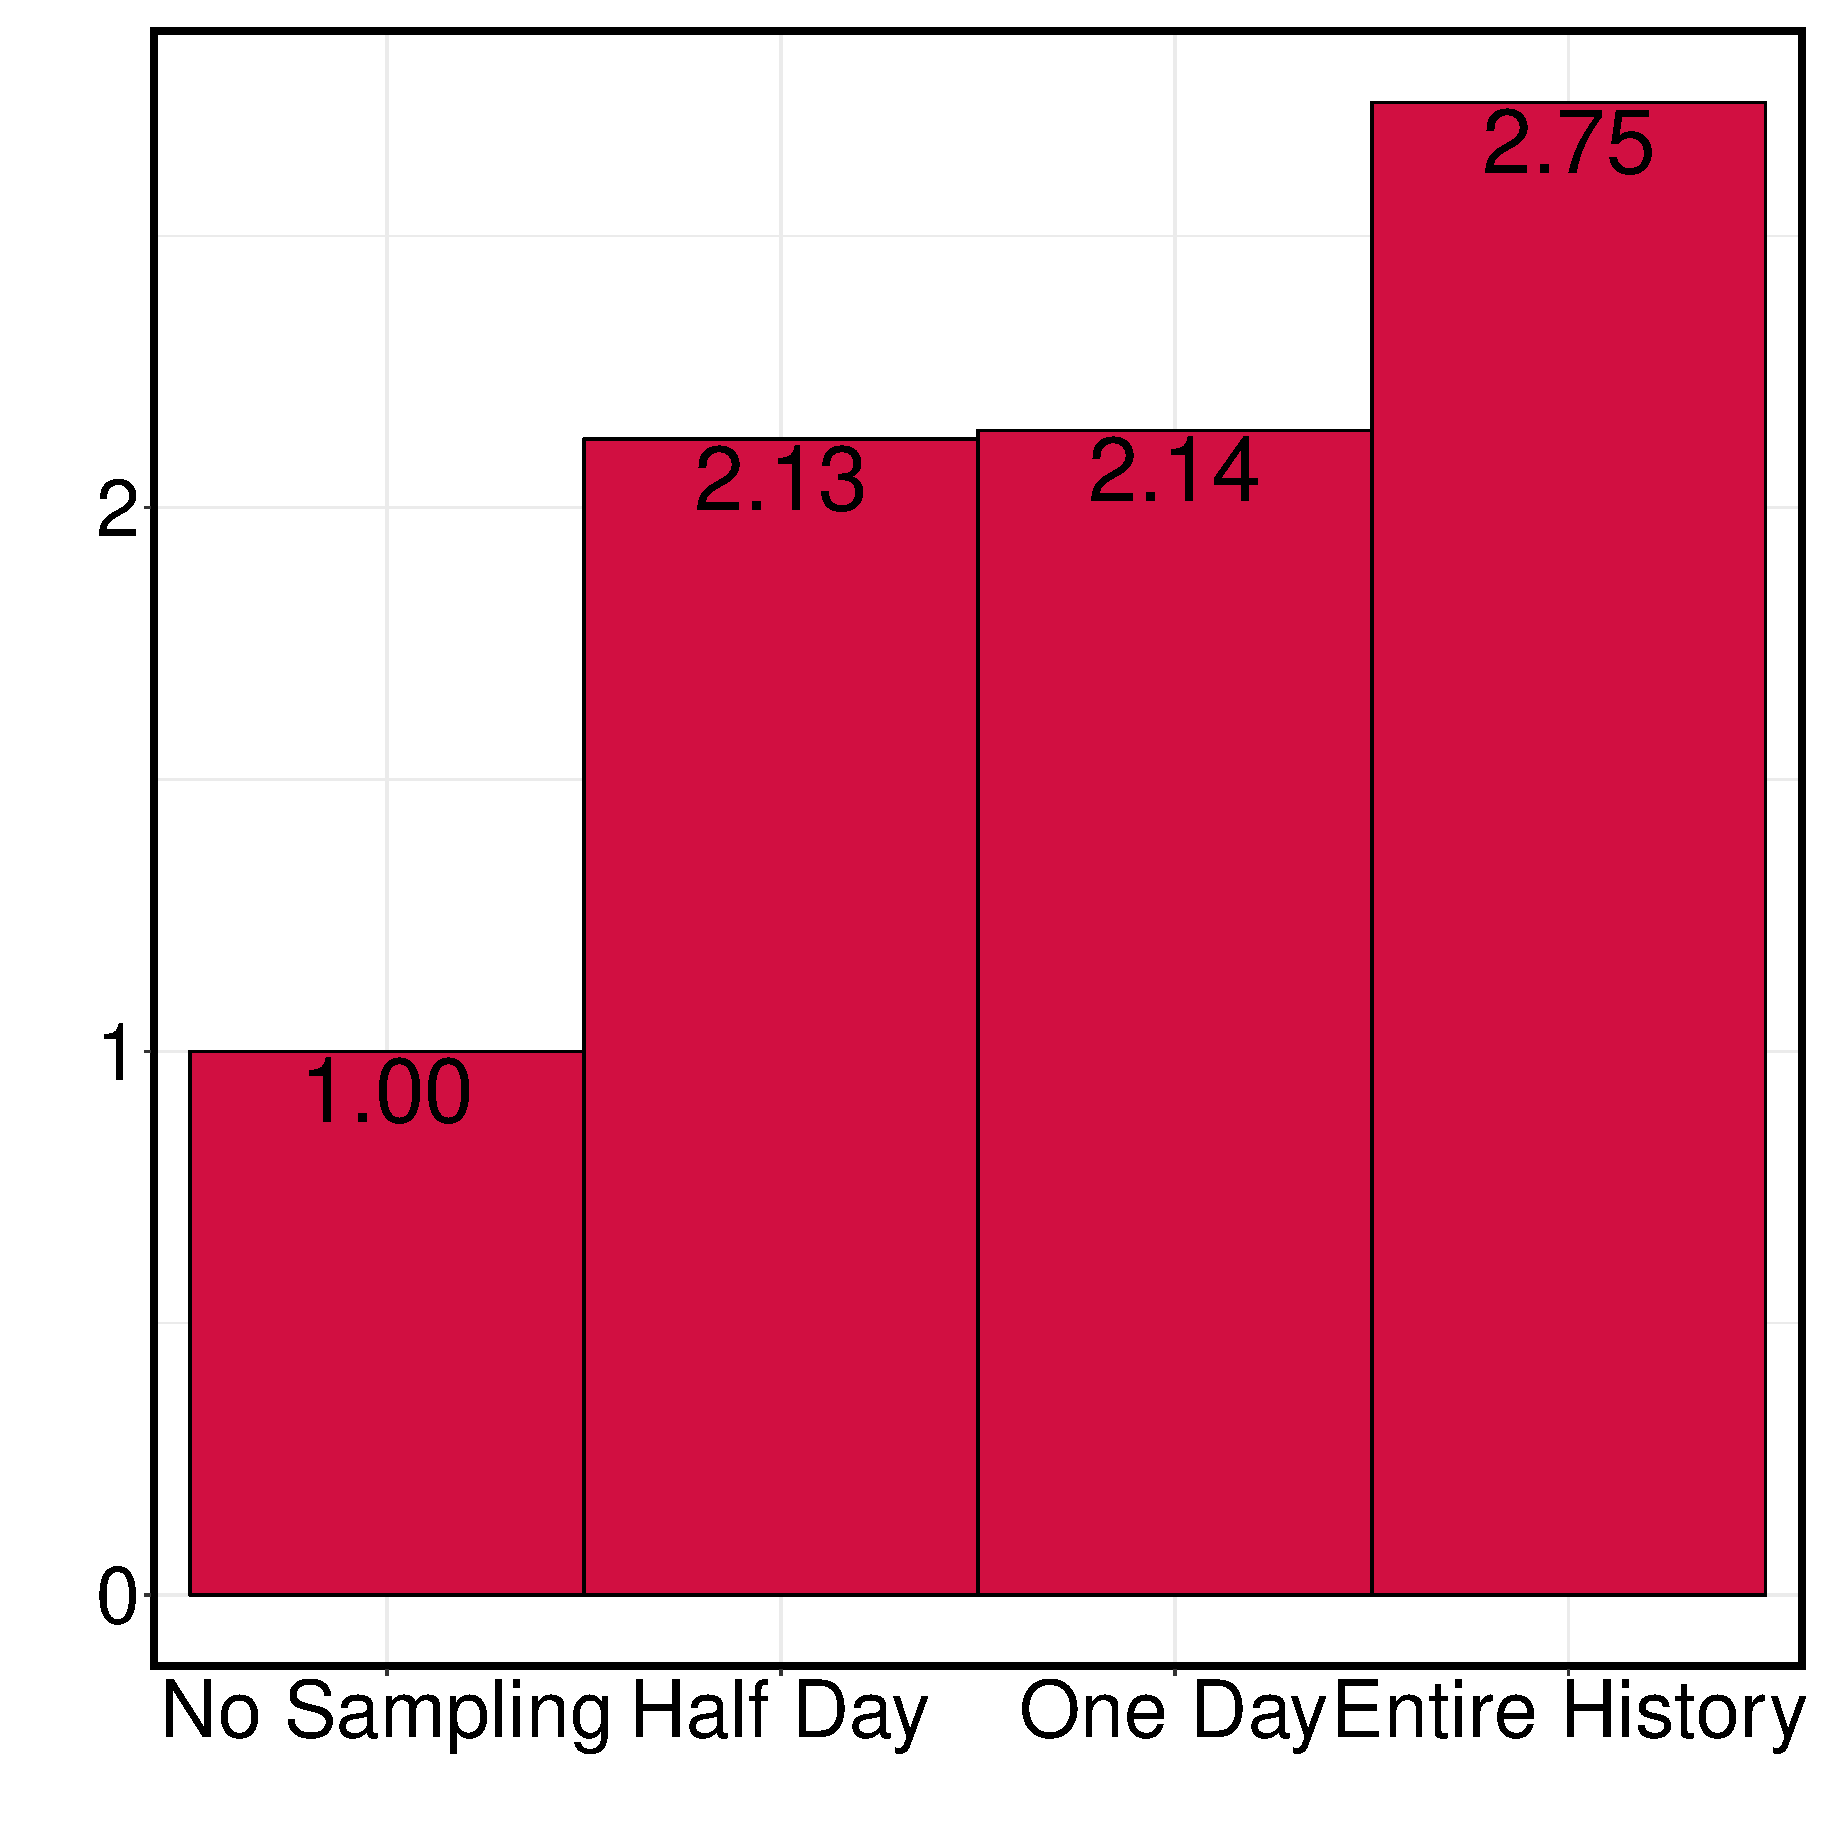
\includegraphics[width=\columnwidth]{../images/experiment-results/criteo-sampling-data-experiment.eps}
\caption{Data processing time}
\label{fig:sampling-mode-data-time}
\end{subfigure}
\vspace{2mm}
\caption{Slowdown factor of different sampling approaches}
\label{fig:sampling-mode-time}
\end{figure}

Figure \ref{fig:sampling-mode-time} shows the effect of different sampling operations on the training time of the pipeline.
Figure \ref{fig:sampling-mode-total-time} shows that using the time-based sampling (intervals of one and half a day) and simple random sampling (the entire history) increases the total training time by a factor of $2.13$ to $2.73$ compared to when no sampling is performed.
However, the slowdown in training time is not due to the sampling operations.
To demonstrate this, for each sampling method, we also capture the amount of time the deployment platform spends in processing the data after the sample is provided by the data manager.
Data processing includes applying the pipeline transformations and training the model.
Figure \ref{fig:sampling-mode-data-time} show the slowdown in data processing time when using different sampling methods.
The slowdown factor for both data processing and the total time is almost identical.
Therefore, the increase in time is not due to the sampling operation.
After the sampling is performed, more data will be processed by the proactive trainer, which increases the total time.

This demonstrates the ability of the data manager to provide samples from the data without incurring overhead on the deployment platform.
The data manager uses a partitioning technique to store the incoming data in a manner that searching and sampling them does not require a scan of the data.
When a sample is required, the data manager directly samples from the list of the data partitions that fall within the range of the required time interval.

\subsection{Scheduling Policy}
In this section, we analyze the scheduling policy of our deployment platform.
In our prototype, we simulated 2 days of continuous training of Criteo data using Apache Spark.
Since the streaming component of Apache Spark requires a fixed interval for executing mini batches, we set out to analyze the effect of our scheduling policy analytically.

Figure \ref{fig:scheduling-policy-time} shows the actual execution time of every proactive training throughout the simulation.
The execution time of the proactive training ranges from $23$ to $53$ seconds.
In order for the scheduler component to effectively schedule proactive training, it requires the prediction latency, prediction throughput, and a user-defined slack parameter.
In our estimation, we use a slack parameter of $10$.
We estimate the throughput and latency based on the time it takes for the deployment platform to predict the labels of the evaluation dataset.
The evaluation dataset contains 2 million data points.
The deployment platform is queried using the evaluation dataset every minute and requires $15$ seconds to return the predictions in the worst case scenario (when the evaluation dataset is stored on disk). 
This amounts to a latency of $7 * 10 ^ {(-6)}$ seconds (7.5 micro seconds) and a throughput of $34,000$ requests per second.

Based on above parameters, the scheduler computes the scheduling intervals for every execution of the proactive training.

\begin{figure}[h!]
\centering
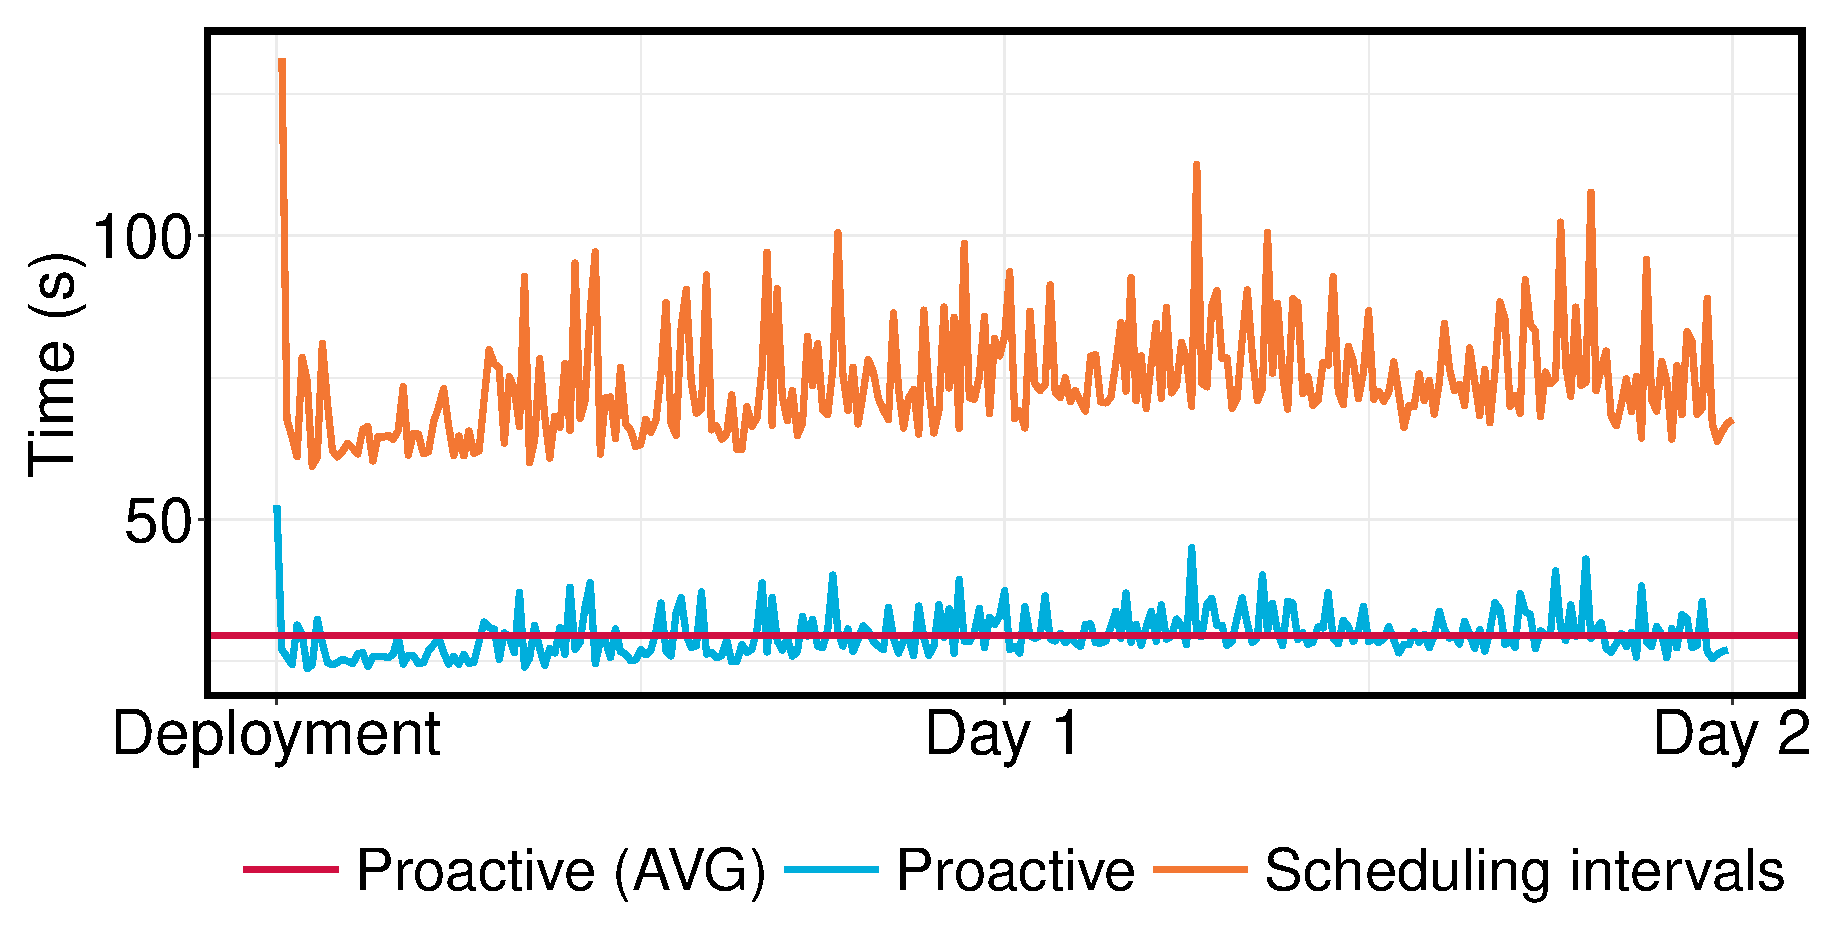
\includegraphics[width=\columnwidth]{../images/experiment-results/criteo-scheduling-experiment.eps}
\caption{Analysis of scheduling policy}
\label{fig:scheduling-policy-time}
\vspace{2mm}
\end{figure}

Using the slack parameter, we can guide the scheduler to increase or decrease the scheduling intervals of the proactive training.
The slack parameter allows for the deployment platform to accommodate surges in the incoming prediction requests and new training data.
In scenarios where sudden surges are expected (e.g., online stores), we recommend a large slack parameter (recommended value is $10$). 


\subsection{Model Freshness}\label{subsec:model-freshness}
We measure the model freshness by two metrics: rate of proactive training execution and rate of new features.
The rate of the proactive training execution is determined by the scheduling rate.
Performing more frequent training results in models that can adapt to changes in the data more rapidly.

To evaluate the model freshness in terms of the rate of new features, we use the feature encoder to determine the number of new features that arrive at the system.
In the Criteo pipeline, the feature encoder is used to transform the categorical features into binary indicator variables.

Figure \ref{fig:criteo-feature-discovery} shows the feature size over time for the first 5 days after deployment of the Criteo pipeline.
The initial training data (Day 0) only contains a small portion of all the unique categorical features of the Criteo dataset.
The rate of incoming new features is close to 30,000 per minute and  around 45 million new features are generated everyday.

\begin{figure}[h!]
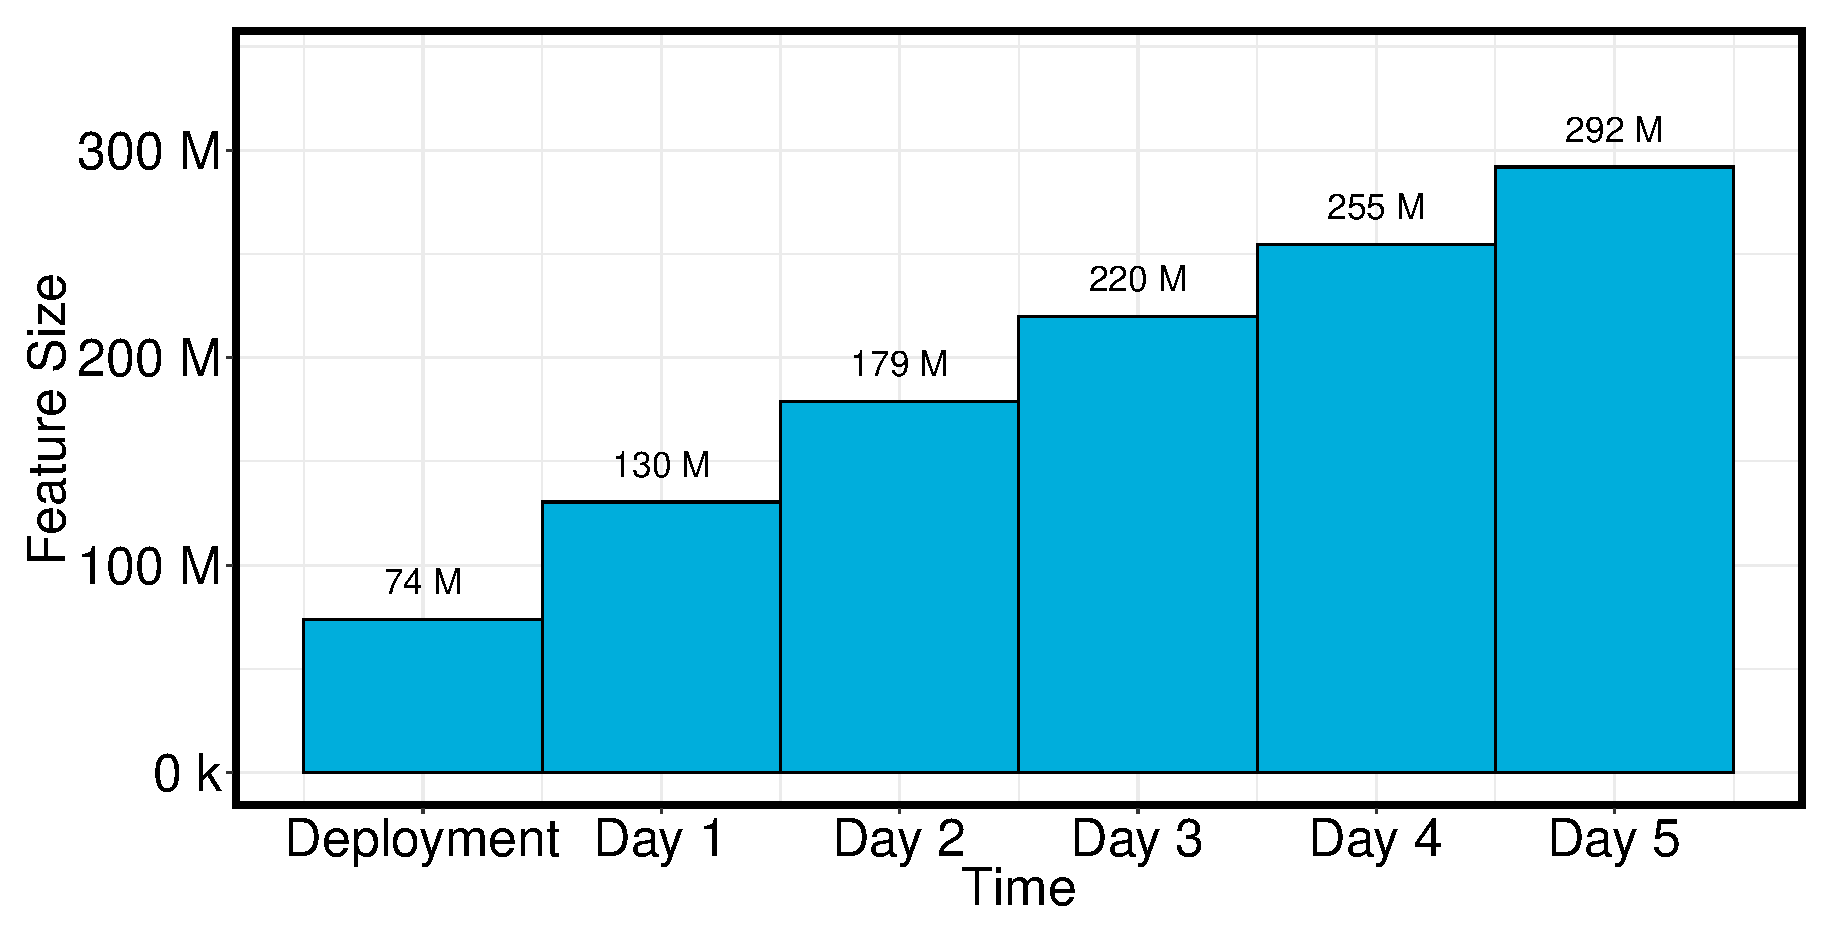
\includegraphics[width=\columnwidth]{../images/experiment-results/criteo-feature-discovery-experiment.eps}
\caption{Criteo categorical feature size over time}
\label{fig:criteo-feature-discovery}
\end{figure}

Using our continuous training approach, we update the pipeline as soon as the new features become available.
During the next scheduled proactive training, the model is updated using these new features.
As a result, the deployed pipeline is able to answer prediction queries that may contain the same set of features more accurately.
Using a daily training approach, any unseen features that arrive at the system are dropped before a prediction is made.

\subsection{Proactive Training}\label{subsec:proactive-training}
In this section, we evaluate the quality of the deployed model.
Figure \ref{fig:loss-proactive-vs-daily} shows the logistic loss of the continuous training and periodical approaches on the Criteo pipeline.

\begin{figure}[h!]
\centering
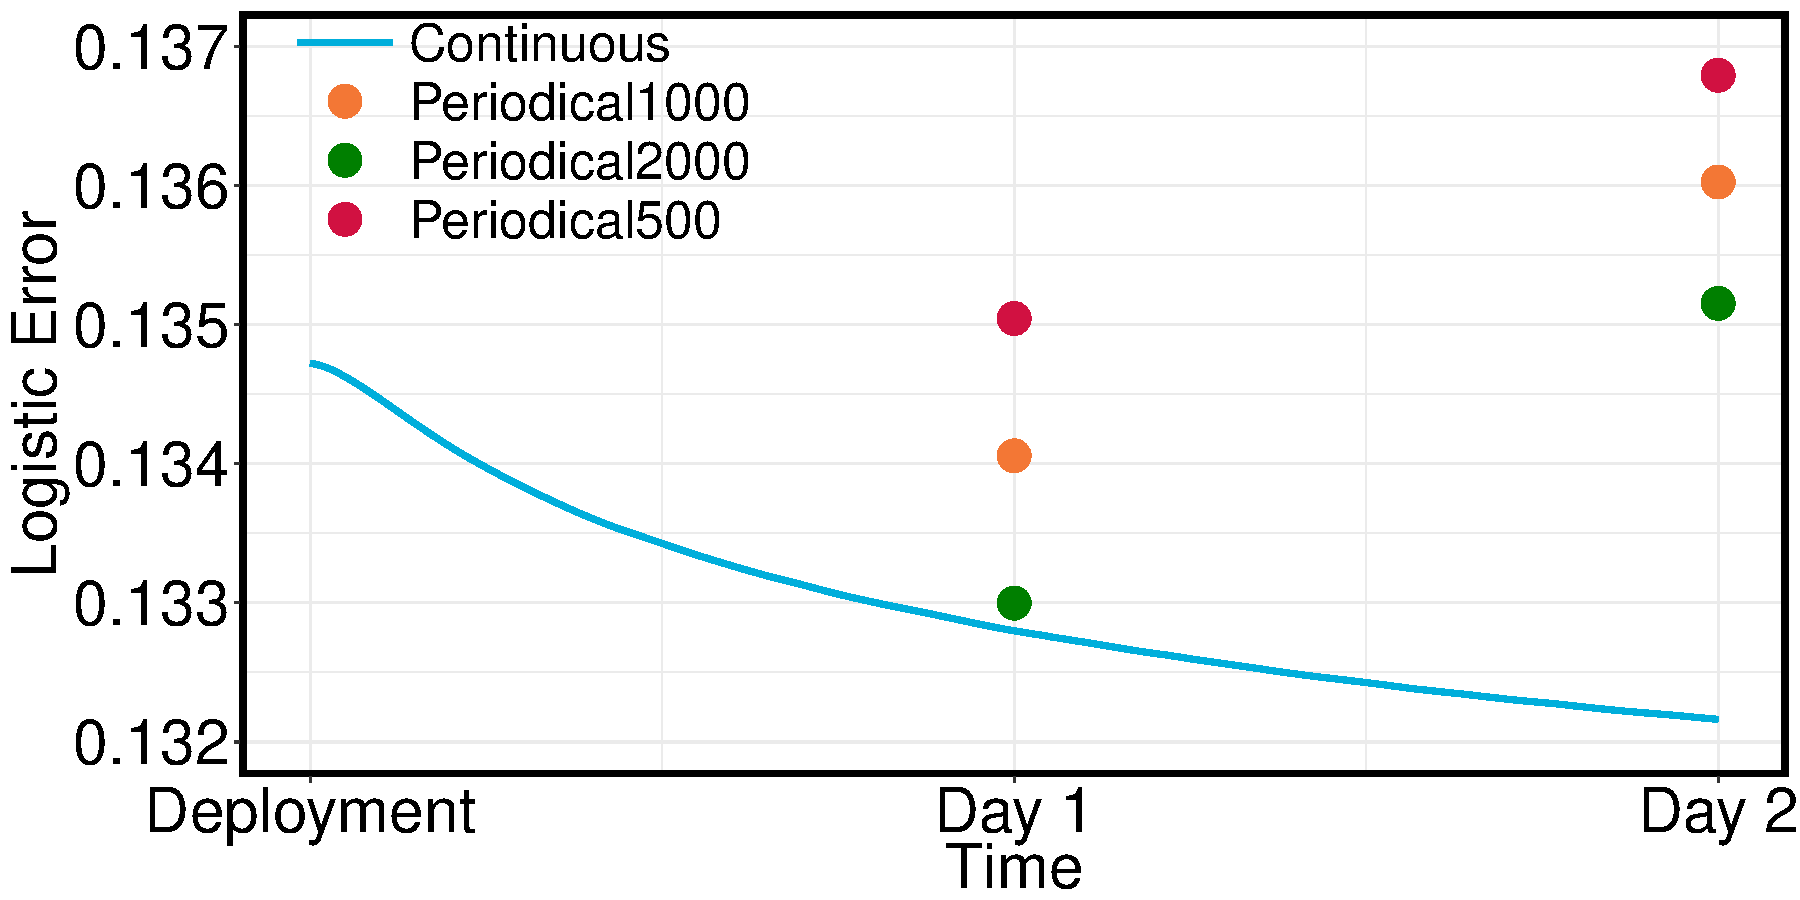
\includegraphics[width=\columnwidth]{../images/experiment-results/criteo-proactive-training.pdf}
\caption{Model quality for different deployment approaches}
\label{fig:loss-proactive-vs-daily}
\vspace{2mm}
\end{figure}

After the deployment, the continuous training updates the pipeline and trains the model using the incoming training data.
The incoming data contains both unseen training observations and new features, as described in experiment \ref{subsec:model-freshness}.
The continuous training approach trains the model over this data within a short period of time which results in a higher quality and fresher model when compared to the periodical training approach.

To measure the performance of the periodical training approach, we train the model at the end of every day of the simulation.
The initial training and periodical training use the same set of parameters.
We use Adam learning rate adaptation technique and a sampling rate of $0.1$ for training the initial and periodical training of the pipeline.

The initial deployed model converges after 500 iterations.
However, after Day 1, the amount of the stored data is doubled, and training the model for $500$ iterations results in a model that has an error rate of $0.002$ higher than the initial model.
Due to the larger number of data points, the periodical training has to train the model longer in order to achieve a lower error rate.
To decrease the error rate of the model further, we train the model for up to $2000$ iterations.
Our experiment shows that continuous training still outperforms periodical training after $2000$ iterations.
The error rate of the model trained using continuous training is $1.6\%$, $0.9\%$, and $0.15\% $ lower than a model trained using the periodical training with $500$, $1000$, and $2000$ iterations respectively at the end of Day 1 of the simulation.

We observe a similar behavior for the second periodical training.
Because of the large training dataset after the second day of the simulation, the model requires a longer training period to converge.
After two days of training, the continuous training approach results in an error rate that is smaller than the error rates of a model trained using $500$, $1000$, and $2000$ iterations by $3.4\%$, $2.8\%$, and $2.2\%$.

This experiment shows that the continuous training of a machine learning pipeline decreases the error rate while still producing fresher models when compared to the periodical training of the pipeline.

It has to be noted that the poor performance of periodical training after each day, can be alleviated by more advanced training methods or better parameter selection for the underlying SGD optimization algorithm.
In this experiment, we demonstrate that using the same set of parameters (learning rate and sample size), we are able to achieve a lower error rate by using the continuous training approach.
In a real deployment scenario, when the quality of the model degrades after the periodical training, either the model is discarded or it is trained for a longer period of time using a more sophisticated training algorithm, while the existing model continuous to answer prediction requests.

\subsection{Total Training Time}
In this section, the total training time for continuous and periodical deployment approaches are measured.
The total training time includes the time spent in pre-processing the training data using the pipeline components and training the model.
For periodical training, we train the model for 500 iterations even though the experiment in Section \ref{subsec:proactive-training} demonstrated that the error rate of such a model is larger than the continuous approach by $1.6\%$.

Figure \ref{fig:training-time-deployment} shows the total training time of the Criteo pipeline for different deployment approaches.
Using continuous training, the time spent in data processing and model training is smaller than that of periodical training by a factor of $5$.
This is due to the large amount of redundant data processing and model training that exists in the periodical training approach.
In the periodical training, the underlying pipeline is trained from scratch every day, which includes ingesting the data, performing the data transformation steps of the pipeline and finally training the model using the transformed data.
However, in continuous training, the pipeline is incrementally updated when new data arrives at the system.

The total training time can be further reduced in the continuous training approach by switching on the online statistics update and materialization optimizations.
Figure \ref{fig:training-time-optimization} shows the effect of each optimizations on the continuous training approach.
By enabling online statistics update, the pipeline components are updated when new training data becomes available.
Therefore, the proactive trainer does not need to update pipeline components and proceeds to transform the data directly.
Enabling the online statistics update optimization reduces the total training time by a factor of $3$.
Moreover, enabling both online statistics and materialization allows the proactive trainer to skip the data processing part of the pipeline completely and directly proceeds to the model training, which only accounts for a small fraction of the pipeline.
Our experiment shows that enabling both online statistics update and materialization reduces the total training time by a factor of $18$, from $142$ minutes of training, when no optimizations are used, to $8$ minutes, when both optimizations are switched on.

\begin{figure}[h]
\begin{subfigure}{\columnwidth/2}
\centering
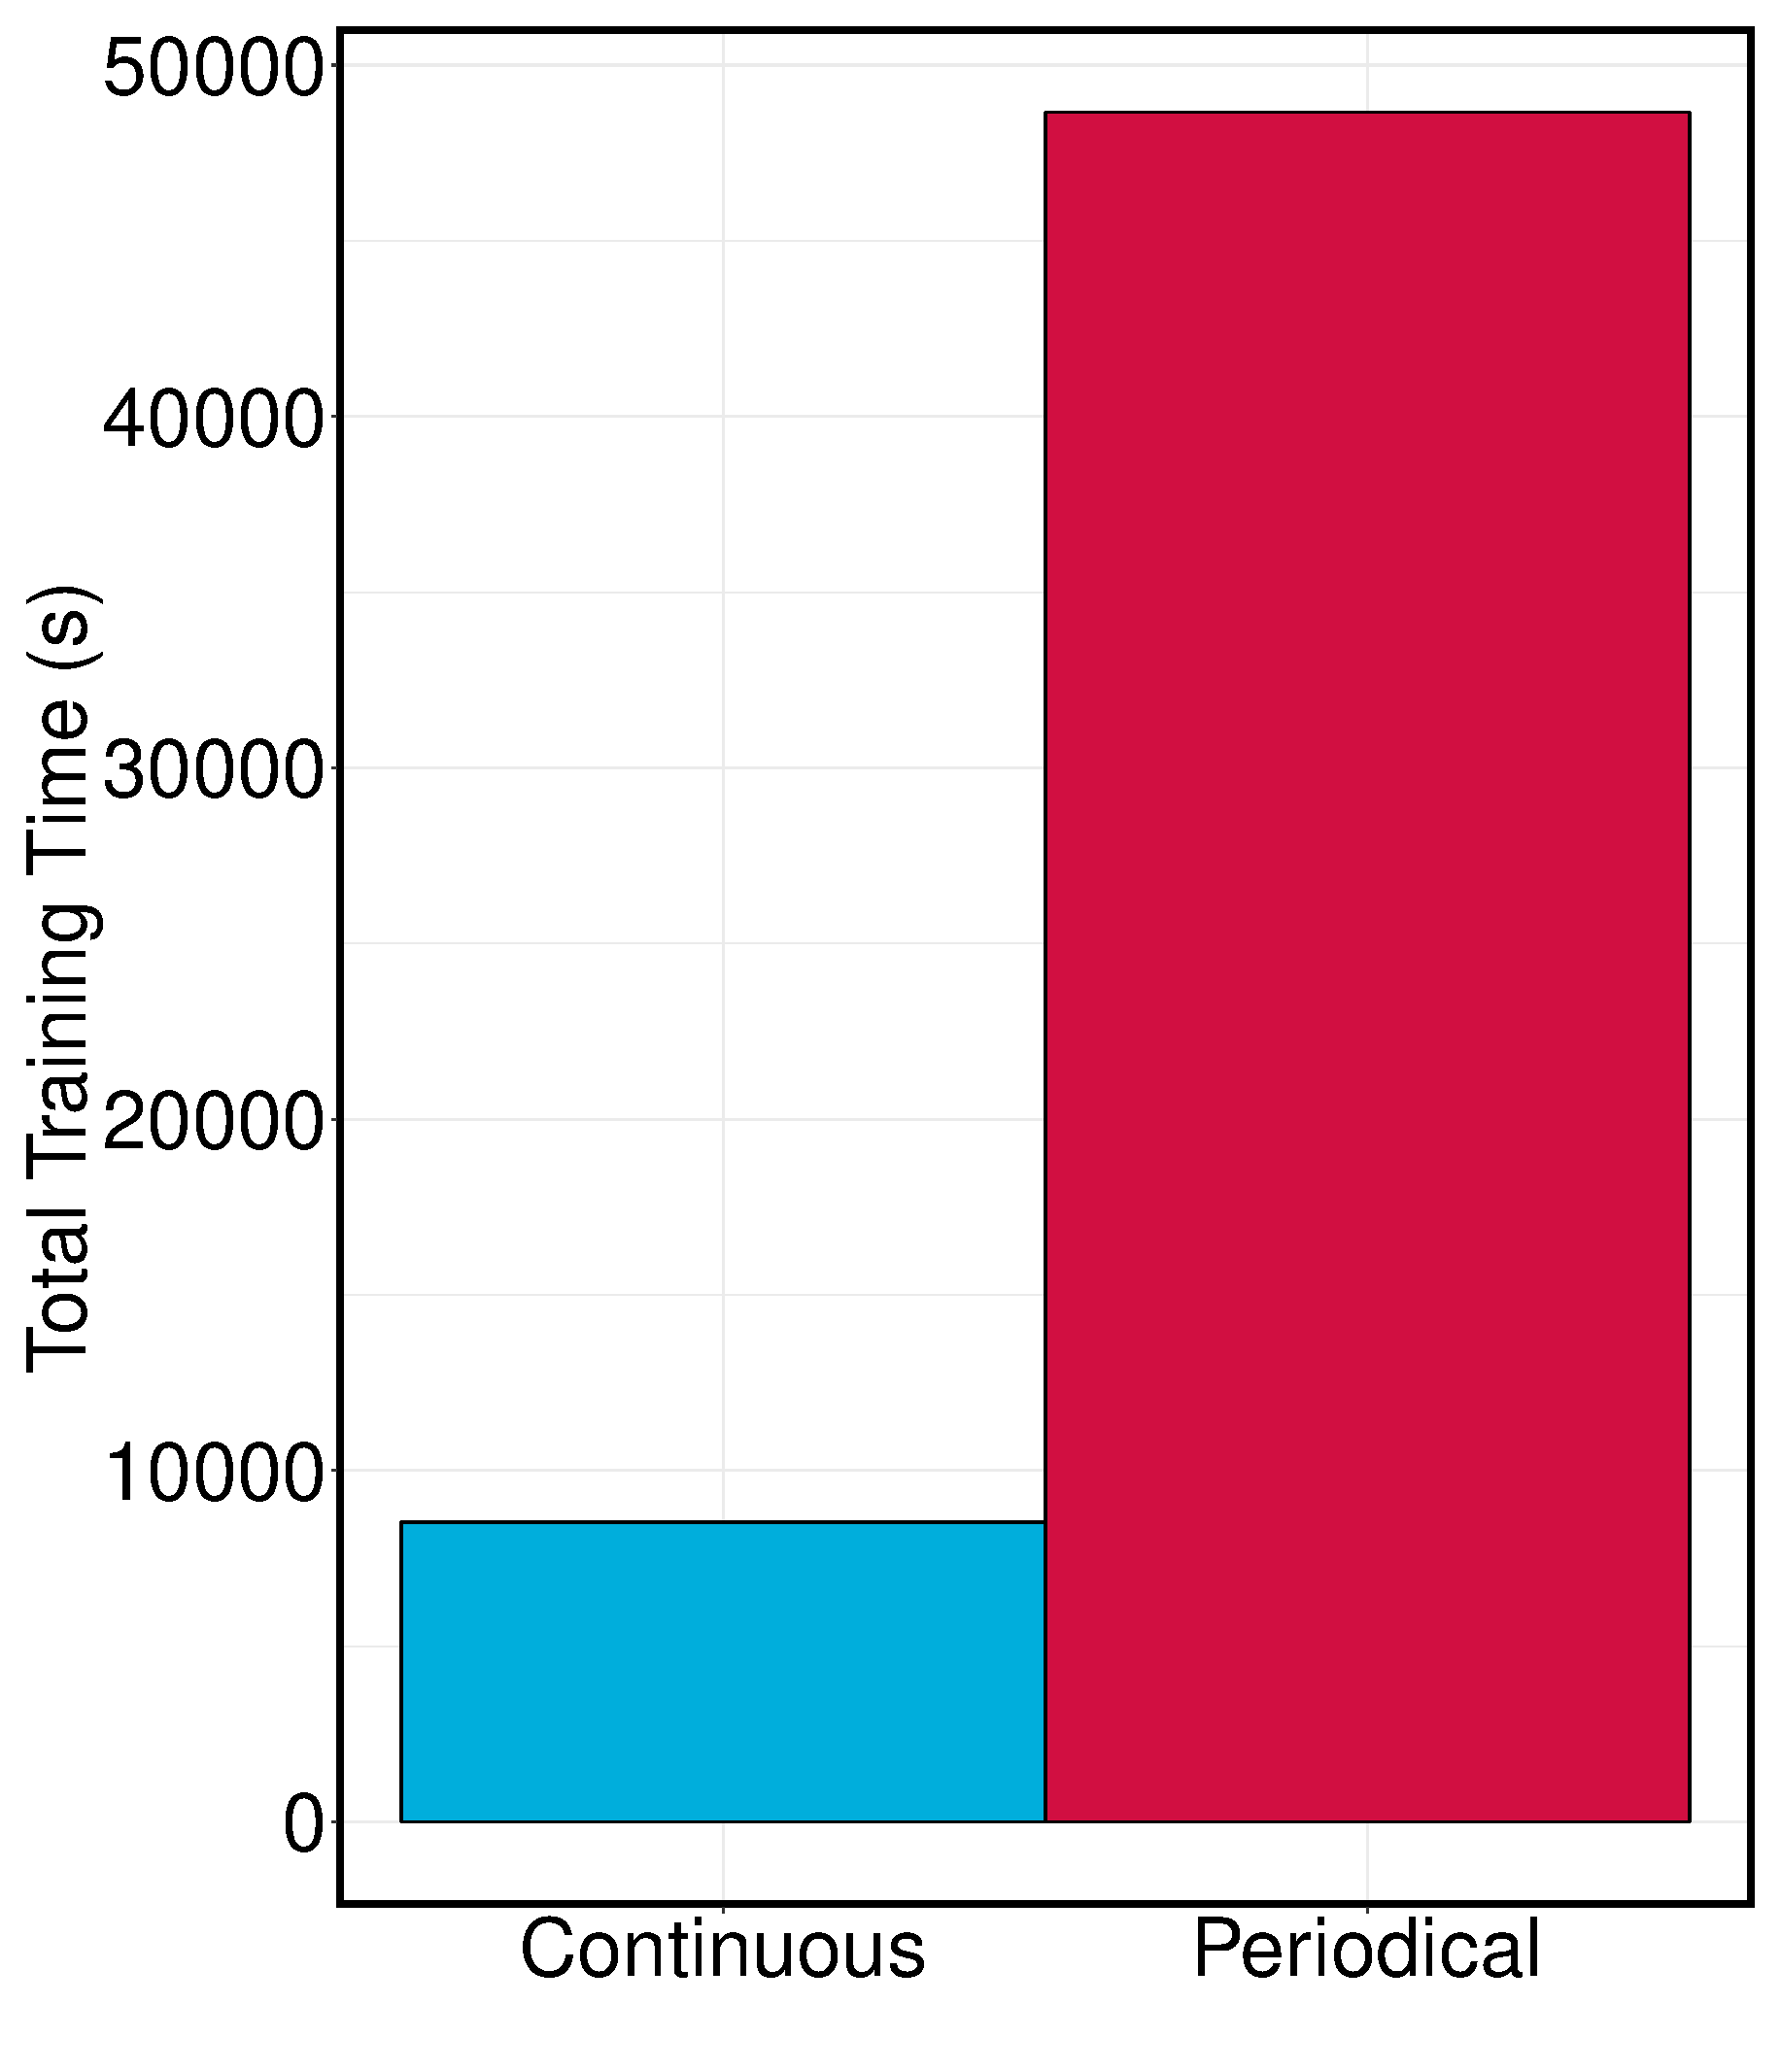
\includegraphics[width=\columnwidth]{../images/experiment-results/criteo-training-time-deployment-types-experiment.eps}
\caption{Deployment Approaches}
\label{fig:training-time-deployment}
\end{subfigure}%
\begin{subfigure}{\columnwidth/2}
\centering
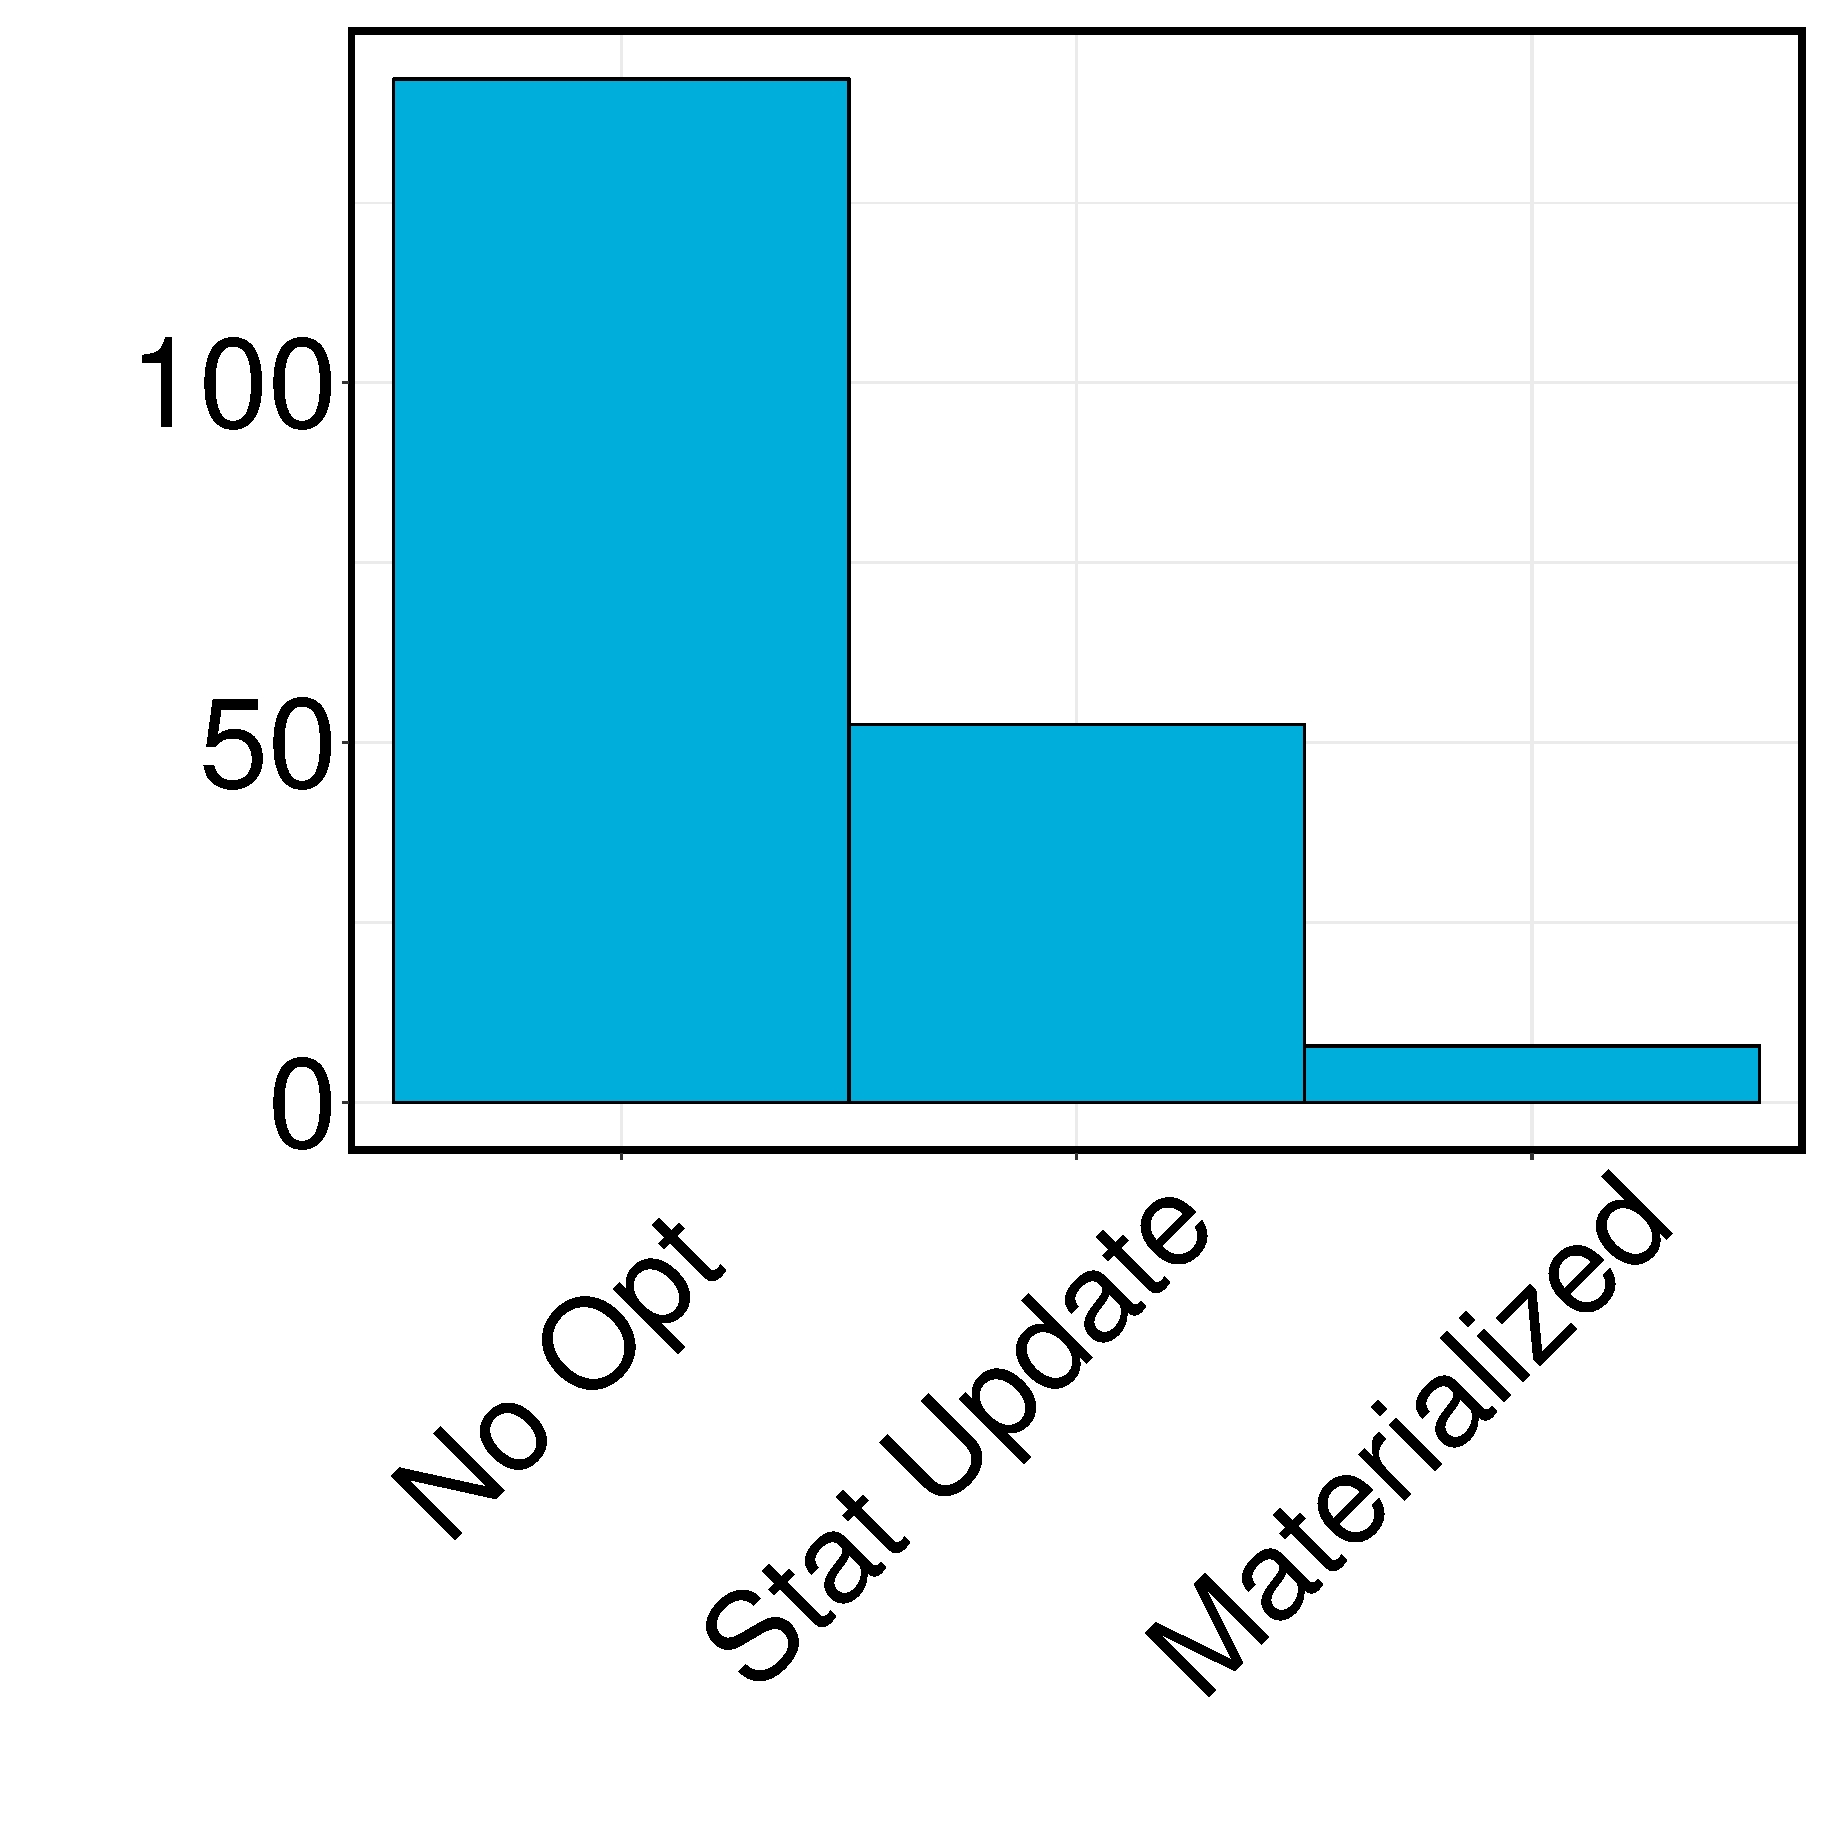
\includegraphics[width=\columnwidth]{../images/experiment-results/criteo-training-time-optimizations-experiment.eps}
\caption{Optimizations}
\label{fig:training-time-optimization}
\end{subfigure}
\vspace{2mm}
\caption{Total training time for different deployment approaches (with optimizations enabled)}
\end{figure}

One possible problem with the materialization optimization is the amount of space required to store the materialized dataset.
Depending on the type of the data processing, the size of the materialized data may increase.
In our experiments, the input data is a combination of Integer and String values, however, after the pre-processing steps of the Criteo pipeline, the data is transformed to large vectors of Double.
As a result, the size of the materialized data increases by a factor of 2.

\subsection{Discussion} \label{subsec:discussion}
Our experiments show that our continuous training approach outperforms periodical training of deployed models and pipelines.
By using proactive training we manage to reduce the average error rate by $1.6\%$.
The frequent updates that the continuous training approach applies to the deployed model is the main reason for the reduction in error rate.
As the amount of the existing data increases after each time interval, periodical training requires more training iterations and more advanced techniques to train a model with an acceptable error rate.
Continuous training does not face the same issue and the error rate of the model decreases when using the continuous training approach, as demonstrated by the experiments.
The continuous training approach enables the model to adapt to the recently unseen data faster and allows the model to be updated with new features.
In contrast to the continuous training, in periodical training, new features are only discovered after each training interval (e.g., 1 day for the Criteo pipeline).
As a result, the deployment platform discards the newly available features when answering prediction requests until the next training.

The continuous training approach reduces the total training time by a factor of $5$ after two days of training.
Moreover, the online statistics computation and data materialization optimizations reduce the total training time by 2 orders of magnitude over the state-of-the-art deployment approaches.
After the model is deployed, the training time for the continuous training approach stays constant as the frequency of proactive training remains the same.
However, periodical training has to process larger datasets at the end of each time interval which leads to the large difference in total training time between continuous and periodical training.

Proactive training is an extension of the SGD optimization algorithm, where during each scheduled training an optional sample of the historical data and the newly available training data are combined and used to train the deployed model in-place.
Therefore, tuning proactive training is similar to the process of tuning the SGD algorithm.
In our experiments, we show that the learning rate adaptation technique that works best with SGD during the offline training also results in the lowest error rate when used in the proactive training.

We demonstrate how different sampling approaches (simple random sampling, time-based sampling, and no sampling) affect the quality of the model.
To perform efficient time-based sampling, the data manager uses a partitioning technique that stores the incoming data in partitions and assigns timestamps to each partition.
Our experiments show that using the data partitioning technique, we can effectively provide samples from different time intervals without incurring an overhead on the deployment platform.
However, while the sampling operations themselves do not incur any overhead, the extra amount of data that is generated as the result of the sampling increases the proactive training time.
To alleviate the issue, we propose a scheduling policy that dynamically adapts to both the rate of the incoming prediction requests and the time required for executing a proactive training.
We show that our scheduling policy can effectively execute the proactive training and adapt to the changes in the rate of the incoming data, the prediction latency, the proactive training time, and the sudden data surges.





